\begin{abwframe}
\node[anchor=north west,inner sep=0pt,outer sep=0pt] at (498.652,-25.651) {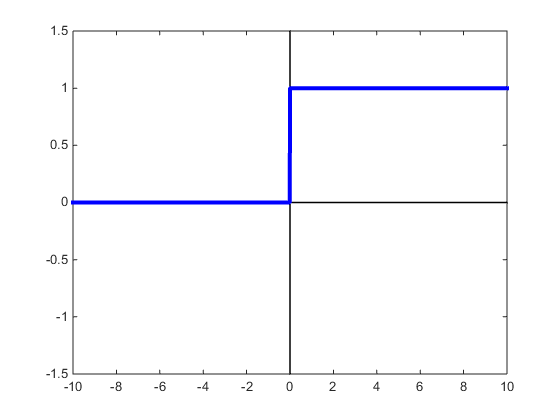
\includegraphics[width=420bp,height=315bp]{assets/source/slide-17-object-001.png}};
\node[anchor=north west,inner sep=0pt,outer sep=0pt] at (40.625,-55.791) {\begin{minipage}[t][69.584bp][c]{878.75bp}\setlength{\parindent}{0pt}\setlength{\parskip}{0pt}{\TimesNR\fontsize{44}{49.28}\selectfont\color{cBC0031}\bfseries\raggedright Activation Functions\par}\end{minipage}};
\node[anchor=north west,inner sep=0pt,outer sep=0pt] at (40.625,-158.857) {\begin{minipage}[t][299.652bp][c]{878.75bp}\setlength{\parindent}{0pt}\setlength{\parskip}{0pt}{\TimesNR\fontsize{24}{26.88}\selectfont\color{c000000}\raggedright A perceptron produces output \ensuremath{z}=\ensuremath{h}  \ensuremath{\mathbf{w}} \ensuremath{T} \ensuremath{\mathbf{x}} .\par}{\TimesNR\fontsize{14}{15.68}\selectfont\color{c000000}\vphantom{Ag}\par}{\TimesNR\fontsize{24}{26.88}\selectfont\color{c000000}\raggedright One choice for the activation function \ensuremath{h}: \\the step function.\par}{\TimesNR\fontsize{24}{26.88}\selectfont\color{c000000}\raggedright  \ensuremath{h} \ensuremath{a} =  0, if \ensuremath{a}<0 1,if \ensuremath{a}\ensuremath{\ge}0  \par}{\TimesNR\fontsize{14}{15.68}\selectfont\color{c000000}\vphantom{Ag}\par}{\TimesNR\fontsize{24}{26.88}\selectfont\color{c000000}\raggedright The step function is useful for providing some intuitive examples.\par}{\TimesNR\fontsize{24}{26.88}\selectfont\color{c000000}\vphantom{Ag}\par}{\TimesNR\fontsize{24}{26.88}\selectfont\color{c000000}\raggedright It is not useful for actual real-world systems.\par}{\TimesNR\fontsize{16}{17.92}\selectfont\color{c000000}\raggedright \hspace*{28bp}\makebox[12bp][l]{\textbullet}Reason: since it is not differentiable, it does not allow optimization via gradient descent, a very powerful method to find the ‘optimal weights’ given a training data set. \par}\end{minipage}};
\node[anchor=north west,inner sep=0pt,outer sep=0pt] at (56.693,-499.702) {\begin{minipage}[t][11.952bp][c]{324bp}\setlength{\parindent}{0pt}\setlength{\parskip}{0pt}{\TimesNR\fontsize{10}{11.2}\selectfont\color{c7F7F7F}\raggedright Analytics for a Better World Lecture 2\par}\end{minipage}};
\node[anchor=north west,inner sep=0pt,outer sep=0pt] at (880.898,-499.702) {\begin{minipage}[t][11.952bp][c]{22.409bp}\setlength{\parindent}{0pt}\setlength{\parskip}{0pt}{\TimesNR\fontsize{10}{11.2}\selectfont\color{c7F7F7F}\bfseries\raggedleft 17\par}\end{minipage}};
\end{abwframe}
